% !Mode:: "TeX:UTF-8"
\documentclass[twoside]{CARDCDef/CARDC}%使用Biber处理参考文献
%\documentclass[twoside,Biber]{CARDCDef/CARDC}%使用Biber处理参考文献

\usepackage{CARDCDef/MyDef}

\makeatletter

%封面大标题
%若自动换行处导致分割词义,可使用\newline命令手动换行,勿使用命令\\换行
\renewcommand{\CARDC@ArtTitle}{中国空气动力研究与发展中心硕博论文模板}
%封面大标题
%若自动换行处导致分割词义,可使用\newline命令手动换行,勿使用命令\\换行
\renewcommand{\CARDC@ArtBigTitle}{中国空气动力研究与发展中心硕博\newline 论文模板}
%封面日期
\renewcommand{\CARDC@ArtSubmitDate}{二零一六年六月}
%导师名字
\renewcommand{\CARDC@FirstTutorName}{梅长苏}
%导师职称
\renewcommand{\CARDC@FirstTutorPost}{宗\hspace{1em}主}
%是否有副导师,有为字母:Y,没有为字母:N
\renewcommand{\CARDC@WithTwoTutor}{Y}
%副导师名字
\renewcommand{\CARDC@SecondTutorName}{飞\hspace{1em}流}
%副导师职称
\renewcommand{\CARDC@SecondTutorPost}{副宗主}
%密级
\renewcommand{\CARDC@SecretLevel}{公开}
%学生名字
\renewcommand{\CARDC@StudentName}{张\hspace{1em}三}
%学号
\renewcommand{\CARDC@StudentID}{}
%专业
\renewcommand{\CARDC@StudentMajor}{武林纷争研究}
%研究方向
\renewcommand{\CARDC@ResearchDirection}{琅琊榜排名}
%硕士还是博士,硕士写上:硕,博士写上:博
\renewcommand{\CARDC@MasterOrDoctor}{博}

%文章大标题英文英文
%若自动换行导致句子不美观,可使用\newline命令手动换行,勿使用命令\\换行
\renewcommand{\CARDC@ArtBigTitleEN}
{Thesis Template for China Aerodynamics Research and Development Center}
%文章的提交日期英文
\renewcommand{\CARDC@ArtSubmitDateEN}{June\hspace{1em}2016}
%导师名字英文
\renewcommand{\CARDC@FirstTutorNameEN}{Changshu Mei}
%副导师名字英文
\renewcommand{\CARDC@SecondTutorNameEN}{Liu Fei}
%学生名字英文
\renewcommand{\CARDC@StudentNameEN}{San Zhang}

\makeatother

%添加参考文献数据库
\addbibresource{bib/ref.bib}

\renewcommand{\bibsetup}{}

\begin{document}

    %中英文封面、独创性声明页
    \maketitle

\frontmatter

    %致谢
    \begin{AbstractCN}
本文是中国空气动力研究与发展中心硕博毕业论文模板示例文件。本模板由L.Y.创建,适用于撰写硕士和博士学位论文。本示例文件介绍了本模板的基础用法外。

\ArtKeywordsCN{气动中心;学位论文; \LaTeX 通用模板;硕士;博士}
\end{AbstractCN}

\begin{AbstractEN}
This is CARDC thesis template for master and doctor user's guide. 
The template is created by L.Y. This document provided the usage of the template.

\ArtKeywordsEN{CARDC; Thesis; \LaTeX{} Template; Master; PhD}
\end{AbstractEN}


    \tableofcontents

\mainmatter

    %正文各个章节
    \chapter{引\hspace{1em}言}

本模板的面向对象不包括对\LaTeX 知识完全不了解之人,特别不适合%
不愿付出适当时间来学习\LaTeX 知识的人。如果您是\LaTeX 新手,本人%
推荐您阅读一些入门文档,比如“lshort”,该文档有社区翻译的中文版本%
《一份不太简短的\LaTeXe 介绍》,您可以从互联网很轻松的找到该文件。%
如果您更加愿意阅读书籍来获得相应的知识,常见的中文书籍有%
陈志杰等\scite{陈志杰LaTeX}编写的《\LaTeX 入门与提高》,但该书涉及%
的知识部分已经过时,且该书作者年纪已大,所以该书也不会继续更新了。%
值得推荐的入门书籍是由刘海洋\scite{刘海洋LaTeX}编写的《\LaTeX 入门》,%
该书作者(LeoLiu)活跃于\CTeX 论坛,是主要板块的版主,同时刘海洋在知乎上%
关于\LaTeX 知识也有许多值得参考的回答,该书的好处是可以让你快速了解必须%
的\LaTeX 知识,同时拓展视野。若您对\LaTeX 知识已有了解,但是涉及不深,%
本人推荐您阅读胡伟\scite{胡伟LaTeX}编写的《\LaTeXe 完全学习手册》,该书%
对常见的\LaTeX 知识做了比较全面的总结,对一些常见的宏包也有介绍,是一本%
不错的工具书籍,可供随时查阅。如果您的\LaTeX 水平已经相当高了,这部分介绍%
可以完全忽略之。如果您问\LaTeX 知识仅止于此吗?答案显然是否定的。例如,%
《The \LaTeX Companion》一书介绍了许多宏包的使用,\TeX 系统作者的书籍%
《The \TeX\ Book》等介绍了更初级的\TeX 命令等。\LaTeX 知识尤其是\TeX 知识%
有时候总是令人困惑的,例如\TeX 中命令的展开方式和时机等,本人疑惑得早已放弃治疗了,%
希望\LaTeX3正式版可以早日推出,让这些事情变得更加简单。

\begin{figure}[h]
  \centering
  % Requires \usepackage{graphicx}
  
\includegraphics[width=0.2\textwidth]{pic/book/ChenZhiJie.jpg} \quad
  
\includegraphics[width=0.2\textwidth]{pic/book/LiuHaiYang.jpg} \quad
  
\includegraphics[width=0.2\textwidth]{pic/book/HuWei.jpg}   \quad
  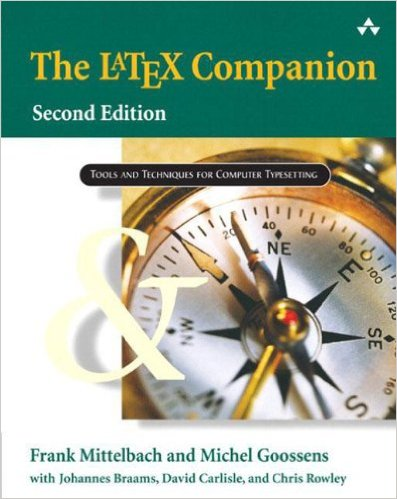
\includegraphics[width=0.2\textwidth]{pic/book/LaTeXCompanion.jpg}
  \caption{\LaTeX 中英文书籍}
\end{figure}

关于本模板的使用,\textbf{您需要的\LaTeX 知识相当少},本文接下来会一一介绍如何使用之。%


\section{软件环境}
\subsection{软件安装}
本文只针对Windows环境,至于Linux环境,本人默认Linux用户能够轻松配置使用之。%
为了快速上手,许多人会选择安装\CTeX 套装,该套装在%
\url{http://www.ctex.org/CTeXDownload} 页面下载,请选择安装%
CTeX\_2.9.2.164\_Full.exe (1.31G)版本,虽然该套装已停止更新,%
但是我们可以通过该套装自带的包更新器更新相应的宏包,而且即使不联网更新,%
该版本也已基本涵盖了我们常用的宏包。%
在这里,本人还是推荐您安装TeXLive,%
该套装的宏包通常比较新。本模板在TeXLive 2015下编译完成,%
本人不保证其在\CTeX 套装的兼容性。接下来,本人假设您已经安装好了以上其中一个版本。%


\subsection{编辑器}
这里采用\CTeX 套装默认的WinEdt,该编辑器专门针对\LaTeX,如果您安装了\CTeX 套装,那么%
该编辑器已经安装好了。如果使用的是TeXLive,那么也可以另外下载该编辑器安装,%
虽然WinEdt是付费软件,但是\dots,没有但是。%
关于更多编辑器的介绍,例如Vim等,您可以去维基百科或者知乎上搜索,有许多%
相应的介绍。关于WinEdt的基本配置和使用,请您阅读本模板附带的图文说明文档%
《第一次使用LaTeX?读我》。接下来,本人默认您已经基本熟悉WinEdt的使用了。


\section{注意事项}
\begin{itemize}
  \item \textbf{本模板的放置路径不含中文或其他乱码字符。}原因是使用Biber编译参考文献时,%
  需要用到管理员权限,而一键编译的脚本,在转换工作路径时,如果含有例如中文,%
  会导致无法正确转换。总而言之,您就用英文就万事大吉了,例如本人的放置路径为:\\
  \verb"F:\WorkDocument\CARDC-Thesis-LaTeX-Template"。

  \item \textbf{图片等资源的文件名请使用英文},确保没有惊喜。
\end{itemize}

\section{问题反馈}
虽然被人已经尽力测试,但是仍不免有不足之处,如果发现有何问题,可以向本人反馈。

    \chapter{模板介绍}
\section{包含的主要文件}
\begin{itemize}
\itemsep=0pt \parskip=0pt
\item \textbf{main.tex:}位于根目录下,是本模板的主要文件。
\item \textbf{bib文件夹:}包含的是参考文献的bib数据库。%
\item \textbf{CARDCDef文件夹:}是本模板的格式设置文件,其中CARDC.cls是
本模板格式的主要设置文件,CARDCTitlePage.sty文件定义了本模板的中英文扉
页和版权声明页,YYBib.sty文件定义了参考文献格式。一般情况下,这三个文件请勿修改。
\item \textbf{chapter文件夹:}是本模板章节内容放置处。
\item \textbf{pic文件夹:}放置了本模板用的图片。
\item \textbf{Script文件夹:}编译调用的脚本文件。
\end{itemize}

\subsection{main.tex文件}
您毕业论文的各项信息请根据注释部分的提示填写即可。

\subsection{ref.bib文件}
在bib文件夹下的ref.bib文件是本模板使用的参考文献数据库。该数据类型可以%
使用其他文献管理软件生成,见本模板附带的图文说明文档《第一次使用LaTeX?读我》。%

\subsection{MyDef.sty文件}
如果您在使用该模板的过程中,需要用到该模板没有导入的宏包或者增加自定义命令,%
可以在导言区增加,或者在CARDCDef文件夹下的MyDef.sty文件中添加,\textbf{本人推荐您%
在MyDef.sty文件中添加,方便统一管理。}

\subsection{Compile.bat}
Windows下的批处理文件,实现一键编译,在文件里面可以切换参考文献后台处理程序,%
如果使用切换至Biber,\textbf{请以管理员权限运行该脚本}。

\subsection{Clean.bat}
Windows下清理临时文件的批处理文件。

\subsection{Makefile}
在Linux环境下(Linux系统或者Cygwin环境),可以使用make工具编译。

\subsection{章节内容}
章节内容包含在chapter文件夹中,已有的是
\begin{itemize}
\itemsep=0pt \parskip=0pt
\item \textbf{abstract.tex:}是中英文摘要。
\item \textbf{appendix.tex:}是附录内容,如果没有附录内容,在main.tex中将该部分%
    导入注释掉。%
\item \textbf{thanks.tex:}是致谢部分。
\item \textbf{1.tex,2.tex:}是本说明文档的第一、二章内容。
\end{itemize}

如果您增加新的章节,请使用UTF-8编码格式,并在main.tex中使用include命令导入即可。%
关于如何将编码格式转为UTF-8,见本模板附带的图文说明文档《第一次使用LaTeX?读我》。%
本人推荐您直接复制chapter目录下的.tex文件,改为需要的名字并导入,然后在里头直接%
书写内容即可。

    \chapter{使用演示}

\section{插入公式}
\LaTeX 可以输出漂亮的公式,但是还是要注意细节才能使公式完美,%
例如输入积分公式:
\begin{equation}
 \int_{a}^{b} f(x) dx,\quad \int_a^b f(x) \mathrm{d}x,\quad \int_a^b f(x)\, \mathrm{d}x
\end{equation}
您是否注意到差别了呢?这里需要注意使用直体d且要注意微小距离,其代码为:
\begin{Verbatim}[]
\int_a^b f(x)\, \mathrm{d}x
\end{Verbatim}

再来输入一个稍微复杂一些的公式:
\begin{equation}
  p_r(x) = \sum_{m=0}^{k} \sum_{j=0}^{m-1}
  v_{i-r+j} \Delta x_{i-r+j} \frac{\sum\limits_{l=0 \atop l \leq m}^{k}
  \prod\limits_{q=0 \atop q \neq m,l}^{k} \Big( x -x_{i-r+q-\frac12} \Big)}
  {\prod\limits_{l=0 \atop l \neq m}^{k} \Big(x_{i-r+m-\frac12} - x_{i-r+l-\frac12} \Big)}
\end{equation}
您可能会觉得,输入一个这样的公式会有多麻烦,其实,如果您熟悉了\LaTeX 命令,%
看到该公式之后,输入起来其实较为简单,照着别人给出的源码输入反而会更加困%
难。

通过自定义命令,可以大幅提高输入效率,例如,本人在MyDef.sty提供了几个命令:%

\begin{itemize}
\itemsep=0pt \parskip=0pt
  \item \verb"\opd"和 \verb"\opD":分别表示直体d和直体D。
  \item \verb"\piandao":偏导数。
  \item \verb"\daoshu":使用d的导数。
  \item \verb"\Daoshu":使用D的导数。
\end{itemize}

\begin{equation}
  \piandao{u}{x},\ \piandao[2]{v}{y^2},\ \piandao[2]{w}{x \partial y},
  \ \daoshu{u}{t},\ \daoshu[2]{u}{t^2},\ \Daoshu{u}{t},\ \Daoshu[2]{u}{t^2}
\end{equation}
以上公式的代码为:
\begin{Verbatim}[]
\piandao{u}{x},\ \piandao[2]{v}{y^2},\ \piandao[2]{w}{x \partial y},
\ \daoshu{u}{t},\ \daoshu[2]{u}{t^2},\ \Daoshu{u}{t},\ \Daoshu[2]{u}{t^2}
\end{Verbatim}

利用它们来输入流体介质运动的动量方程:
\begin{equation}
  \rho \left( \piandao{v_i}{t} + v_j \piandao{v_i}{x_j}\right)
  = -\piandao{p}{x_i} + \piandao{e_{ij}}{x_j}
\end{equation}
其源码是:
\begin{Verbatim}[]
  \rho \left( \piandao{v_i}{t} + v_j \piandao{v_i}{x_j}\right)
  = -\piandao{p}{x_i} + \piandao{e_{ij}}{x_j}
\end{Verbatim}
通过自定义命令,使得源码看起来稍微简洁了许多,也可以简化输入。

\section{插入图片}
您可能需要掌握的知识是:
\begin{itemize}
\itemsep=0pt \parskip=0pt
  \item minipage环境:可以让一组图片放在同一页上。
  \item subfig宏包:主要用于插入子图,和minipage结合,可达到多种插图效果。
  \item 浮动环境控制:由于插图使用了浮动环境,您需要理解什么是浮动环境,%
  以及 \verb"\clearpage"和 \verb"\newpage"用法的区别,否则图片可能不会出现在%
  你想让它出现的地方。
  \item 图片大小微调:在您基本完成论文之后,如果有些空白您实在无法调整好,%
  可能需要对插图尺寸参数作微调,以达到完美的效果。
\end{itemize}
本节列举一些常见的多图插入用法,具体参见本文档对应处的源码。

\begin{figure}[h]
\begin{minipage}[t]{0.5\textwidth}
  \centering
  
\includegraphics[width=0.9\textwidth]
    {pic/example.png}
  \caption{图a}\label{fig:图a}
\end{minipage}
\begin{minipage}[t]{0.5\textwidth}
  \centering
  
\includegraphics[width=0.9\textwidth]
    {pic/example.png}
  \caption{图b}\label{fig:图b}
\end{minipage}
\end{figure}

\begin{figure}[h]
  \centering
  \subfloat[图形a]{
    \label{fig:PicA}
    
\includegraphics[width=0.4\textwidth]
        {pic/example.png}
  }\quad
  \subfloat[图形b]{
    \label{fig:PicB}
    
\includegraphics[width=0.4\textwidth]
        {pic/example.png}
  }
  \caption{两个并列的子图形}
\end{figure}

\begin{figure}[h]
  \centering
  \subfloat[图形a]{
    \label{fig:PicB}
    
\includegraphics[width=0.4\textwidth]
        {pic/example.png}
  }\\
  \subfloat[图形b]{
    \label{fig:PicA}
    
\includegraphics[width=0.4\textwidth]
        {pic/example.png}
  }\quad
  \subfloat[图形c]{
    \label{fig:PicB}
    
\includegraphics[width=0.4\textwidth]
        {pic/example.png}
  }
  \caption{三个子图形}
\end{figure}

\begin{figure}[h]
\begin{minipage}[t]{0.5\textwidth}
    \centering
  \subfloat[图形a]{
    \label{fig:PicA}
    
\includegraphics[width=0.8\textwidth]
        {pic/example.png}
  }\\
  \subfloat[图形b]{
    \label{fig:PicB}
    
\includegraphics[width=0.8\textwidth]
        {pic/example.png}
  }\\
   \subfloat[图形c]{
    \label{fig:PicB}
    
\includegraphics[width=0.8\textwidth]
        {pic/example.png}
  }
  \caption{第一组图}
\end{minipage}
\begin{minipage}[t]{0.5\textwidth}
    \centering
  \subfloat[图形a]{
    \label{fig:PicA}
    
\includegraphics[width=0.8\textwidth]
        {pic/example.png}
  }\\
  \subfloat[图形b]{
    \label{fig:PicB}
    
\includegraphics[width=0.8\textwidth]
        {pic/example.png}
  }\\
   \subfloat[图形c]{
    \label{fig:PicB}
    
\includegraphics[width=0.8\textwidth]
        {pic/example.png}
  }
  \caption{第二组图}
\end{minipage}
\end{figure}

\clearpage

\section{插入表格}
插入表格时,您可能需要对表格参数作出微调,使得表格较为美观。
\begin{table}[h]
\setlength{\tabcolsep}{5mm}%增加列间距
\caption{参数表格}\label{tab:参数表格}
  \centering
\begin{tabular}{|c|c|c|c|c|c|}
  \hline
  % after \\: \hline or \cline{col1-col2} \cline{col3-col4} ...
    & A & B & C & D & E \\\hline
  u & 3 & 1 & 2 & 2.9 & 2.9 \\\hline
\end{tabular}
\end{table}

如果有长表格,您需要使用长表格环境:longtable。

\section{参考文献}
本模板参考文献格式按研部要求定制,研部要求模糊之处,参考了2015年12月1日生效的%
国家标准GB/T 7714-2015\scite{国标2015}。参考文献分成了几类,不同类别对应关系如下:%
\begin{itemize}
\itemsep=0pt \parskip=0pt
  \item \textbf{ARTICLE:}普通文献;
  \item \textbf{BOOK:}书籍;
  \item \textbf{REPORT:}报告;
  \item \textbf{THESIS:}学位论文;
  \item \textbf{PATENT:}专利;
  \item \textbf{PROCEEDINGS:}会议文集;
  \item \textbf{INPROCEEDINGS:}会议文集析出文献;
  \item \textbf{ONLINE:}网络文献。
\end{itemize}
如果您还有其余类别需要输入,请您反馈给本人,本人继续按规范添加。

\subsection{ARTICLE}
ARTICLE类别中英文示范如下,注意到中文文献需要另外说明语言选项,%
即需要加入条目“\verb"language = {chinese},"”,\textbf{所有中文条目都需要加入该选项},%
每个选项都以英文逗号结束。%
第一项“\verb"Ellzy1995"”和“\verb"李晓东1999"”是标签条目,供引用命令使用,%
引用方式为“\verb"\scite{Ellzy1995}"”或“\verb"\scite{李晓东1999}"”。如果同时引用%
多个条目,逗号分隔即可,例如,“\verb"\scite{Ellzy1995,李晓东1999}"”。系统会自动根据%
参考文献的首次引用顺序按照模板设定好的格式依次插入参考文献列表中。其余各项说明如下:%
\begin{itemize}
\itemsep=0pt \parskip=0pt
  \item author:作者列表,用and分隔,这部分之后还会细说;
  \item title:文献标题;%
  \item journal:是杂志的名称,也可以写成“\verb"journaltitle={...}"”,%
    选其中一种方式即可;
  \item year:是文献的年份;
  \item volume:是文献的卷号;
  \item number:是文献的期号;%
  \item pages:是页码范围,若不写页码,请删除该项,而不是写成“\verb"pages={ },"”。
\end{itemize}

\begin{Verbatim}[]
@ARTICLE{Ellzy1995,
  author = {Robert Clayton and Bj\"orn Engquist},
  title  = {Absorbing boundary conditions for acoustic and elastic wave equation},
  journal= {Bulletin of the Seismological Society of America},
  year   = {1997},
  volume = {67},
  number = {6},
  pages  = {1529-1540},
}
\end{Verbatim}
\begin{Verbatim}[]
@ARTICLE{李晓东1999,
  language =   {chinese},
  author   =   {李晓东 and 张庆红 and 叶瑾琳},
  title    =   {气候学研究的若干理论问题},
  journal  =   {{北京大学学报: 自然科学版}},
  year     =   {1999},
  volume   =   {35},
  number   =   {1},
  pages    =   {101-106},
}
\end{Verbatim}

\subsection{BOOK}
BOOK类各项说明如下:
\begin{itemize}
\itemsep=0pt \parskip=0pt
  \item author:作者列表,用and分隔;
  \item translator:翻译者,用and分隔;%
  \item title:文献标题;%
  \item publisher:出版者;
  \item year:年份;
  \item address:出版地址,也可以写成“\verb"location={...}"”,%
    选其中一种方式即可;
  \item pages:是页码范围。
\end{itemize}
\begin{Verbatim}[]
@BOOK{刘海洋LaTeX,
  language =     {chinese},
  author =       {刘海洋},
  title =        {\LaTeX 入门},
  publisher =    {电子工业出版社},
  year =         {2013},
  address =      {北京},
}
\end{Verbatim}
\begin{Verbatim}[]
@BOOK{哈里森经济2012,
  language =     {chinese},
  author =       {哈里森 and 沃尔德伦},
  translator =   {谢远涛},
  title =        {经济数学与金融数学},
  publisher =    {中国人民大学出版社},
  year =         {2012},
  address =      {北京},
  pages =        {235-236},
}
\end{Verbatim}
\begin{Verbatim}[]
@BOOK{FANX,
  author =       { X Fan and C H Sommers},
  title =        {Food irradiation research and technology},
  publisher =    {Blackwell Publishing},
  year =         {2013},
  edition =      {2},
  address =      {{Ames, Iowa}},
  pages =        {25-26},
}
\end{Verbatim}

\subsection{REPORT}
institution表示机构或学校,其余选项的意义参考BOOK类。
\begin{Verbatim}[]
@REPORT{冯西桥1997,
  language =     {chinese},
  author =       {冯西桥},
  title =        {核反应堆压力管道与压力容器的LBB分析},
  institution =  {清华大学核能技术研究设计院},
  year =         {1997},
  address =      {北京},
}
\end{Verbatim}

\subsection{THESIS}
选项的意义参考BOOK类和REPORT类,这里的institution选项也可以改为school选项,二选其一即可。
\begin{Verbatim}[]
@THESIS{周林2012,
  language =     {chinese},
  author =       {周林},
  title =        {可压缩自由剪切流的线性稳定性及噪声机理研究},
  institution =  {中国科学技术大学},
  year =         {2012},
  address =      {安徽合肥},
}
\end{Verbatim}

\subsection{PROCEEDINGS}
与BOOK类基本相同。
\begin{Verbatim}[]
@PROCEEDINGS{台湾光复2012,
  language =     {chinese},
  author =       {中国社会科学院台湾史研究中心},
  title =        {台湾光复六十五周年暨抗战史实学术研讨会论文集},
  publisher =    {九州出版社},
  address =      {北京},
  year=          {2012},
}
\end{Verbatim}


\subsection{INPROCEEDINGS}
与BOOK类基本相同,只是这里的booktitle是论文集的名字。
\begin{Verbatim}[]
@INPROCEEDINGS{诸叶梅2004,
  language =     {chinese},
  author =       {诸叶梅},
  title =        {浅谈我国科技期刊国际化},
  pages =        {184-186},
  publisher =    {中国科学技术协会},
  year =         {2004},
  address =      {北京},
  booktitle =    {首届科技出版发展论坛论文集},
}
\end{Verbatim}


\subsection{PATENT}
PATENT的各项说明如下:
\begin{itemize}
\itemsep=0pt \parskip=0pt
  \item author:专利的所有者或者申请人;
  \item title:专利名称;
  \item location:是专利的国别;%
  \item number:专利号;
  \item date:专利的公开日期;
\end{itemize}
您可能注意到示范里头的number条目,这个专利的专利号为201220158825,%
为何写成“\verb"2012201588\-2\-5"”,这是因为我引用该专利\scite{张凯军2012Patent}的时候,%
该专利的专利号过长,而系统将其当做一个整体,所以会溢出边界,而“\verb"\-"”是告诉系统,%
如果溢出了的话,你可以在此处折断换行。“\verb"2012201588\-2\-5"”就表示,既可以在2这里%
折断,也可以在5这里折断,系统根据需要自动判断在何处折断可保持美观。如果您发现有类似情况%
都看参照此处理。
\begin{Verbatim}[]
@PATENT{张凯军2012Patent,
  language =     {chinese},
  author =       {张凯军},
  title =        {轨道火车及高速轨道火车紧急安全制动辅助装置},
  location =     {中国},
  number =       {2012201588\-2\-5},
  date =         {2012-04-05},
}
\end{Verbatim}


\subsection{ONLINE}
选项意义如下:
\begin{itemize}
\itemsep=0pt \parskip=0pt
  \item date:更新或修改日期;
  \item urldate:引用日期,该项可选;%
  \item url:访问路径。
\end{itemize}
其余选项参考前面的条目说明。
\begin{Verbatim}[]
@ONLINE{萧钰2012Online,
  language =     {chinese},
  author =       {萧钰},
  title =        {出版业信息化迈入快车道},
  date =         {2012-04-05},
  url  =         {http://www.creader.com/news/20011219/200112190019.html},
}
\end{Verbatim}


\subsection{姓名列表}
中文姓名列表无需过多说明,使用and分割即可,这里主要说一下“歪果仁”的姓名。%
外国人姓名的构成是:first name + 连接词 + last name,first name就是我们所说的%
名,按照著录规则,应该取首字母并大写,last name是我们所说的姓,连接词如von、van、de、la等。%
举个“栗子”,例如,Charles-Jean Étienne Gustave Nicolas de La Vallée Poussin,那么%
名为,Charles-Jean Étienne Gustave Nicolas,缩写为C-J É G N,所以最后著录格式为:
de La Vallée Poussin C-J É G N。这个过程系统会自动处理,您无需费心。另外,西方人名字%
可能还会包含缀字,例如Junior,表示什么一世、二世之类,好吧,本人未遇到过这样的文献,%
如果遇到了您手动处理一下吧。

正常情况下,系统可以自动处理姓名列表,如引用该文献\scite{Ellzy1995},该文献作者为%
Robert Clayton 和 Bj\"orn Engquist,在bib数据库中输入方式见ARTICLE类别的示范,系统%
可以自动处理之。如果您引用的参考文献作者本来就已经是缩写好了的,或者系统不能正确处理,%
您已经手动处理好,那么怎么输入呢?例如,引用的这个文献\scite{FANX},作者名字已经按规定缩写%
好了,那么输入的时候请将名字用大括号括起来,并用and分隔,%
“\verb"author={{Fan X} and {Sommers C H}},"”。原因是,大括号括起来的部分会当
成一个整体。或者您也可以写成:“\verb"author={X Fan and C H Sommers},"”

总结如下:
\begin{itemize}
\itemsep=0pt \parskip=0pt
  \item 正常英文情况:\{Michael Jordan and Dwyane Tyrone Wade\}。
  \item 中文姓名的拼音示范:梅长苏应写为 \{Chang Shu Mei\}。
  \item 手动处理:大括号括起来 \{\{Fan X\}\}或者\{X Fan\}。
  \item 复姓处理:用大括号将复姓括起来 \{Maria \{San Martino\}\},或者%
    用逗号分隔,将姓写在前面\{San Martino, Maria\},推荐前一种方式。
\end{itemize}

关于这部分更多的知识,%
请参考《\LaTeXe 用户手册》附录B中关于参考文献的部分,这本书籍在互联网上很容易下%
载到。

\subsection{Unicode字符}
如果您按照本模板附带的图文说明文档《第一次使用LaTeX?读我》中依次编译的话,.bib数据库中%
是不能包含有\LaTeX 不认识的字符的。例如,É这个字母,您需要按\LaTeX 方式输入为“\verb"{\'E}"”,%
这是因为按照这种方式编译,参考文献是使用BibTeX处理的,%
这种方式无法处理这类Unicode字符(BibTeX无法处理的表现有时是直接忽略该字符,像你没输入一样)。%
如果您不喜欢这种输入方式,喜欢直接输入É这种方式,那么需要用到Biber程序来处理参考文献。%
Biber是处理参考文献的另一个程序,已一起打包至\CTeX 套装中。此时,您在第一遍编译完主文件之后,%
不能点击BibTeX编译参考文献,而是打开命令行,输入命令Biber main即可。本质上,WinEdt上的%
按钮,后台也是按命令行处理的,您甚至可以修改按钮背后的处理方式,详见本模板附带的%
图文说明文档《第一次使用LaTeX?读我》。这一切都太复杂?您还是按\LaTeX 方式输入吧,%
或者根本没有这类Unicode字符那是最好的,或者直接点击根目录下的批处理脚本编译%
(本质上也是命令行),前提是Windows环境变量设置正确,如果正常安装\CTeX 套装,那么环境变量%
就已经设置好了。需要说明的是,在正文中,您可以正常使用Unicode,例如本说明文档中,%
我就是直接输入的É这个字母,而无需输入为“\verb"{\'E}"”。

\subsection{编译方式}
参考文献处理可以使用BibTeX或者Biber,具体说明见本模板附带的图文说明文档%
《第一次使用LaTeX?读我》。

    %....继续增加章节

    %参考文献
    \YYBibAddRefToContent
    \printbibliography

    %附录,无请注释掉
    \appendix
        \chapter{无粘通量特征分解}

\section{一维N-S方程}

\section{二维N-S方程}

\section{三维N-S方程}



\chapter{湍流初场生成}

\section{网格构造}

\section{生成算法}


\backmatter

    %\chapter{Biber测试}

%测试Biber
\begin{refsection}[bib/refForTest.bib]

\nocite{外作者1,外作者2,外作者3,外作者4,外作者5,外作者7,外作者8,外作者9}

\printbibliography[heading=subbibliography,title={Biber测试}]
\end{refsection}


    %硕(博)阶段的成果
    \chapter{攻读博士学位期间的研究成果}

%已接收或已发表的论文
\begin{refsection}

\nocite{周林2012IJA,万振华2012QD}

\printbibliography[heading=subbibliography,title={已接收或已发表的论文}]
\end{refsection}


%准备投递的文章
\begin{refsection}

\nocite{周林1,周林2}

\printbibliography[heading=subbibliography,title={准备投递的文章}]
\end{refsection}

\vspace{8pt}%控制适当的距离

%获得奖励情况
\begin{flushleft}
\sanhao\textbf{获得奖励情况}
\end{flushleft}
呵呵~~

    % 致谢
	
\begin{thanks}

本模板的制作参考了中国科学技术大学的本硕博模板,向该模板制作者表示敬意。

感谢大家对本模板更新工作的支持!

本模板以及本示例文档还存在许多不足之处,欢迎大家测试并及时提供反馈。

\begin{flushright}
L.Y.
\end{flushright}


\end{thanks}
%硕博致谢部分


\end{document}
